\subsection*{Balance general}
\addcontentsline{toc}{subsection}{Balance general}

Según el Banco BBVA \parencite{BBVA05}, \textit{'El balance general o balance de situación de una empresa es un documento contable financiero que refleja la situación económica y patrimonial de la misma en una fecha determinada; lo que en términos contables se conoce como imagen fiel. Este documento, que se elabora periódicamente, permite conocer la situación financiera y patrimonial de una compañía en un momento concreto, pues en él se detallan sus activos, sus pasivos y su capital.'}

La responsabilidad de preparar y presentar estos estados financieros corresponde a la sección administrativa de la empresa. Por lo tanto, nos enfocaremos en el balance general, dentro del cual se ofrece información acerca de la situación financiera de la empresa al final de un período contable.

La información que contiene un balance general se clasifica de tal forma que los usuarios puedan obtener detalles acerca de la liquidez, la fecha de vencimiento de los pasivos, la cantidad de activos asignados a inmuebles, maquinaria y otros equipos, así como la porción de los activos aportada por los propietarios y accionistas.

Estos datos sobre la liquidez de los activos se obtienen al distinguir los activos entre corrientes y no corrientes. Los activos corrientes se componen de efectivo y de los recursos que se espera que se conviertan en efectivo al ser vendidos o consumidos dentro de un año o dentro del ciclo normal de operaciones (el que sea más largo). El ciclo normal de operaciones corresponde al período de tiempo que transcurre entre la compra del inventario, su procesamiento para la venta, la venta de los bienes y el posterior cobro derivado de dichas ventas.

La situación financiera se representa mediante una serie de recursos que pueden ser utilizados por la empresa, denominados activos, y las demandas sobre esos recursos, representadas por los pasivos y el patrimonio neto.

\begin{center}
	\textit{Patrimonio = Activos - Pasivos}
\end{center}

En la tabla \ref{BalanceGeneral} se describen los activos, pasivos y el patrimonio correspondientes a cada año, tomando como punto de partida el año 0 como inversión inicial, de forma que este represente el inicio de los procesos del negocio. Esto se plantea considerando la proyección de ventas, la cual inicia desde el año contable 1 hasta el año 5.

Este balance debe presentarse para la aprobación de la Asamblea General de Accionistas por parte del representante legal, junto con los demás documentos establecidos en el Artículo 446 del Código de Comercio. Dentro del término establecido por la ley, el representante legal remitirá a la Superintendencia, cuando sea el caso, una copia del balance y los anexos que lo justifican y explican, además del acta en la que hayan sido discutidos y aprobados.

\begin{table}[H]
	\centering
	\caption[{Balance general}]{\centering Balance general. \textit{Fuente:} Autores.}
	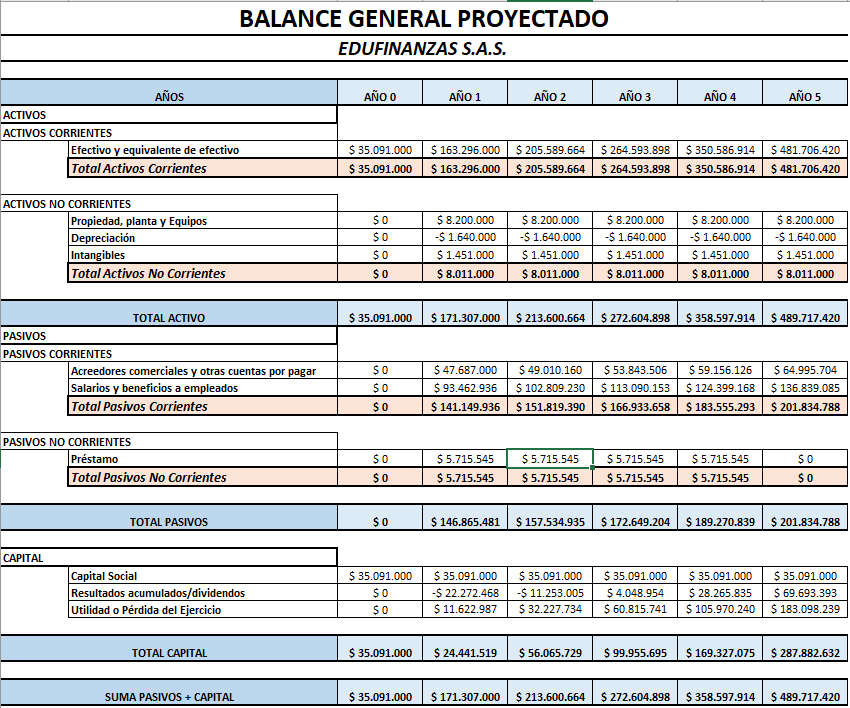
\includegraphics[width=15cm]{Imagenes/BalanceGeneral.png}
	\label{BalanceGeneral}
\end{table}